\documentclass[fleqn,usenatbib]{mnras}

\usepackage{newtxtext,newtxmath}
\usepackage{graphicx}
\usepackage{amsmath}
\usepackage{booktabs}
\usepackage{multirow}
\usepackage{tabularx}
\usepackage{url}
\usepackage{orcidlink}

\title[Calibrating Dyson-sphere selection]{From Dyson-sphere candidates to population constraints: calibrating selection and real-image completeness in Gaia--2MASS--WISE searches}

\author[Zhang]{
Yuzhan Zhang$^{1}$\orcidlink{0009-0000-3121-7972}\thanks{E-mail: wujijiandao2333@163.com}
\\
$^{1}$Independent Researcher, Beijing, China
}

\date{Accepted XXX. Received YYY; in original form ZZZ}
\pubyear{2026}

\begin{document}
\label{firstpage}
\pagerange{\pageref{firstpage}--\pageref{lastpage}}
\maketitle

\begin{abstract}
Mid-infrared searches for partial Dyson spheres can identify sources consistent with stellar obscuration plus thermal waste heat, but candidate counts cannot be converted into occurrence rates without a selection function matched to the candidate operator. We calibrate coupled response terms using a 100-pc Gaia DR3 parent sample cross-matched to 2MASS and AllWISE. A 10-band injection--recovery experiment using 265 real stellar templates and a 220,745-model partial-Dyson library yields a mean photometric recovery of 0.910 across a 54-cell waste-heat grid, conditional on the validation-eligible ten-band sample. Applying Gaia/WISE host cuts to the same 3,000 validation stars gives a source-level joint photometric-plus-host recovery of 0.414, rather than 0.402 from multiplying stage averages. We then inject co-spatial waste-heat flux into real AllWISE W3/W4 images. In a leave-one-host-out analysis, each test star is excluded from empirical PSF construction and morphology calibration. No morphology rejection occurs among 23 independent baseline-clean hosts in either band within the tested unsaturated regime; the one-sided 95 per cent exact lower bound on host-level retention is 0.878 per band and 0.873 jointly for 22 hosts. Retention remains unity when the pseudo-$\chi^2$ feature is removed and under stricter empirical thresholds. We separate image completeness into environmental, detector-response, and conditional morphology terms. Population occurrence can be inferred only when candidate rate, candidate composition, and completeness refer to the same selection operator; the remaining end-to-end terms are not yet calibrated, so we do not report an occurrence rate.
\end{abstract}

\begin{keywords}
extraterrestrial intelligence -- infrared: stars -- methods: statistical -- catalogues -- surveys
\end{keywords}

\section{Introduction}

The thermodynamic argument that sufficiently large-scale stellar-energy use should generate detectable waste heat has motivated searches for Dyson spheres and related technosignatures for more than six decades \citep{Dyson1960}. Early infrared searches used IRAS to identify approximately blackbody-like sources and place whole-sky upper limits on luminous Dyson spheres \citep{Carrigan2009}. The G-HAT programme subsequently developed a broader formalism for Dysonian searches with WISE and Spitzer, emphasizing both the energy-budget interpretation of mid-infrared emission and the importance of natural dust and source confusion as false positives \citep{Wright2014a,Wright2014b,Griffith2015}. Gaia adds precise distances and optical photometry to this infrared search space, enabling complementary tests based on optical dimming and parallax consistency \citep{Zackrisson2018}.

Project Hephaistos brought these ideas to large stellar samples. Hephaistos-I combined Gaia DR2 and AllWISE to set phenotype-dependent upper limits on partial Dyson spheres \citep{Suazo2022}. Hephaistos-II then developed a Gaia DR3--2MASS--WISE candidate pipeline containing SED fitting, quality cuts, image screening with a convolutional neural network, signal-to-noise requirements, and final visual inspection; seven M-dwarfs survived as candidates for follow-up \citep{Suazo2024}. Subsequent observations have reinforced the importance of the image and contamination terms in such a pipeline. Radio imaging and archival diagnostics indicate background contamination for several systems \citep{Ren2024RNAAS,Ren2025,Ren2026}, while JWST/MIRI resolves background galaxies within approximately one arcsecond of two candidates \citep{Zackrisson2026}. The stellar properties of the broader candidate set remain of astrophysical interest even where an artificial interpretation is disfavoured or unresolved \citep{Korn2026}.

The statistical issue considered here is more general than the status of any individual candidate. A candidate-search pipeline is a measurement operator: a real source must first enter the relevant catalogues, retain usable measurements after the technosignature phenotype modifies its SED, survive deterministic astrophysical and catalogue-quality cuts, remain acceptable in the image domain, and then satisfy the final candidate definition. The rate at which a pipeline produces candidates therefore depends on the underlying population and on the pipeline response.

This perspective is standard in survey astronomy. A selection function is the probability that an object with specified properties enters a scientific sample; importantly, the relevant selection function is unique to the sample actually used for inference \citep{EverallDas2020,BoubertEverall2022}. Gaia provides a particularly clear example: subsets defined by reported astrometry, radial velocity, or RUWE cuts have non-trivial selection functions in magnitude, colour, and position \citep{EverallBoubert2022}. Infrared-excess searches face an additional complication because source confusion can generate apparent excesses: in a WISE study of approximately 180,000 Kepler stars, most nominal warm-dust excesses were attributable to background structure or chance alignments rather than circumstellar emission \citep{KennedyWyatt2012}. These precedents motivate treating a Dyson-sphere candidate list as a selected sample rather than as a direct census of the underlying phenotype.

Let
\begin{equation}
r_{\rm cand}=P({\rm candidate}\mid{\rm star})
\end{equation}
be the candidate rate in a specified stellar parent population,
\begin{equation}
\pi_{\rm DS}=P({\rm DS}\mid{\rm candidate})
\end{equation}
be the fraction of admitted candidates belonging to the target phenotype, and
\begin{equation}
C_{\rm DS}=P({\rm candidate}\mid{\rm DS})
\end{equation}
be the completeness of that same candidate operator for the target phenotype. The common-event identity
\begin{equation}
P({\rm DS}\cap{\rm candidate}\mid{\rm star})
=\pi_{\rm DS}r_{\rm cand}
=f_{\rm DS}C_{\rm DS}
\end{equation}
gives
\begin{equation}
f_{\rm DS}=\frac{\pi_{\rm DS}r_{\rm cand}}{C_{\rm DS}}.
\label{eq:selection_inversion}
\end{equation}
Equation~(\ref{eq:selection_inversion}) is elementary probability, not a new statistical theorem. Its practical force comes from the requirement that all three measured quantities refer to the same parent population, phenotype definition, and candidate-selection operator. A candidate rate measured after a final visual screen cannot consistently be divided by a completeness measured only at an upstream photometric stage.

The purpose of this paper is to calibrate and audit several response terms required by equation~(\ref{eq:selection_inversion}), rather than to claim an occurrence rate. We reconstruct a real 100-pc Gaia DR3 parent sample with 2MASS and AllWISE cross-matches, perform partial-Dyson injection--recovery on real stellar SEDs, propagate the same injected hosts through deterministic Gaia/WISE quality cuts, and then test co-spatial waste-heat injection in real AllWISE W3/W4 images. The final image experiment is leave-one-host-out, so a tested star contributes neither to the empirical PSF used to inject it nor to the empirical morphology calibration used to classify it. We additionally audit threshold choice and image-metric dependence. This approach isolates which pieces of the response are currently measured and which remain external-validity limitations.

The contribution is therefore operational rather than a claim to have invented selection-function theory. We make three empirical advances specific to partial-Dyson searches: (i) we measure photometric and host-quality response jointly on the same injected real sources, exposing the bias in multiplying stage-average efficiencies; (ii) we move the image-response experiment from a Gaussian image emulator to real AllWISE intensity, uncertainty, and coverage data with epoch-corrected source positions and leave-one-host-out calibration; and (iii) we separate field-environment rejection, bright-source non-linearity, and conditional morphology retention so that these distinct effects are not compressed into a single ``image completeness'' number. The inferential contribution is to connect these measured response terms to a selection-consistent candidate-to-population inversion while leaving unmeasured terms explicit.

\section{Data, parent sample, and conditioning structure}
\label{sec:data}

\subsection{Gaia DR3 mother sample and cross-matches}

We selected Gaia DR3 sources with parallax greater than 10 mas, corresponding nominally to distances smaller than 100 pc. The resulting mother catalogue contains 574,531 Gaia sources. We intentionally did not pre-clean this catalogue by RUWE, signal-to-noise ratio, or astrophysical-parameter availability: removing problematic sources before defining the response would turn part of the selection process into an undocumented precondition.

The Gaia mother sample was cross-matched separately to 2MASS \citep{Skrutskie2006} and AllWISE \citep{Wright2010,Cutri2013}. Cross-match results were merged locally with left joins so that missing counterparts remained explicit. In the full mother sample, 47.49 per cent have an AllWISE counterpart and 52.36 per cent have a 2MASS counterpart. These raw fractions are not interpreted as Dyson-sphere completeness; the mother catalogue intentionally contains a broad set of Gaia sources that are not all suitable for a ten-band stellar SED analysis.

\subsection{Main-sequence selection}

We defined a broad colour--magnitude main-sequence sample in absolute Gaia $G$ magnitude and $G_{\rm BP}-G_{\rm RP}$ colour. A source is rejected as a giant when
\begin{equation}
M_G<4
\quad\hbox{and}\quad
M_G<7(G_{\rm BP}-G_{\rm RP})-3,
\end{equation}
and rejected as a white-dwarf/high-absolute-magnitude source when
\begin{equation}
M_G>3(G_{\rm BP}-G_{\rm RP})+5.
\end{equation}
We additionally retain $0\le M_G\le13.6$. This produces 250,909 candidate main-sequence stars; 204,613 of them have RUWE $<1.4$. Figure~\ref{fig:cmd} shows the selection.

\begin{figure}
\centering
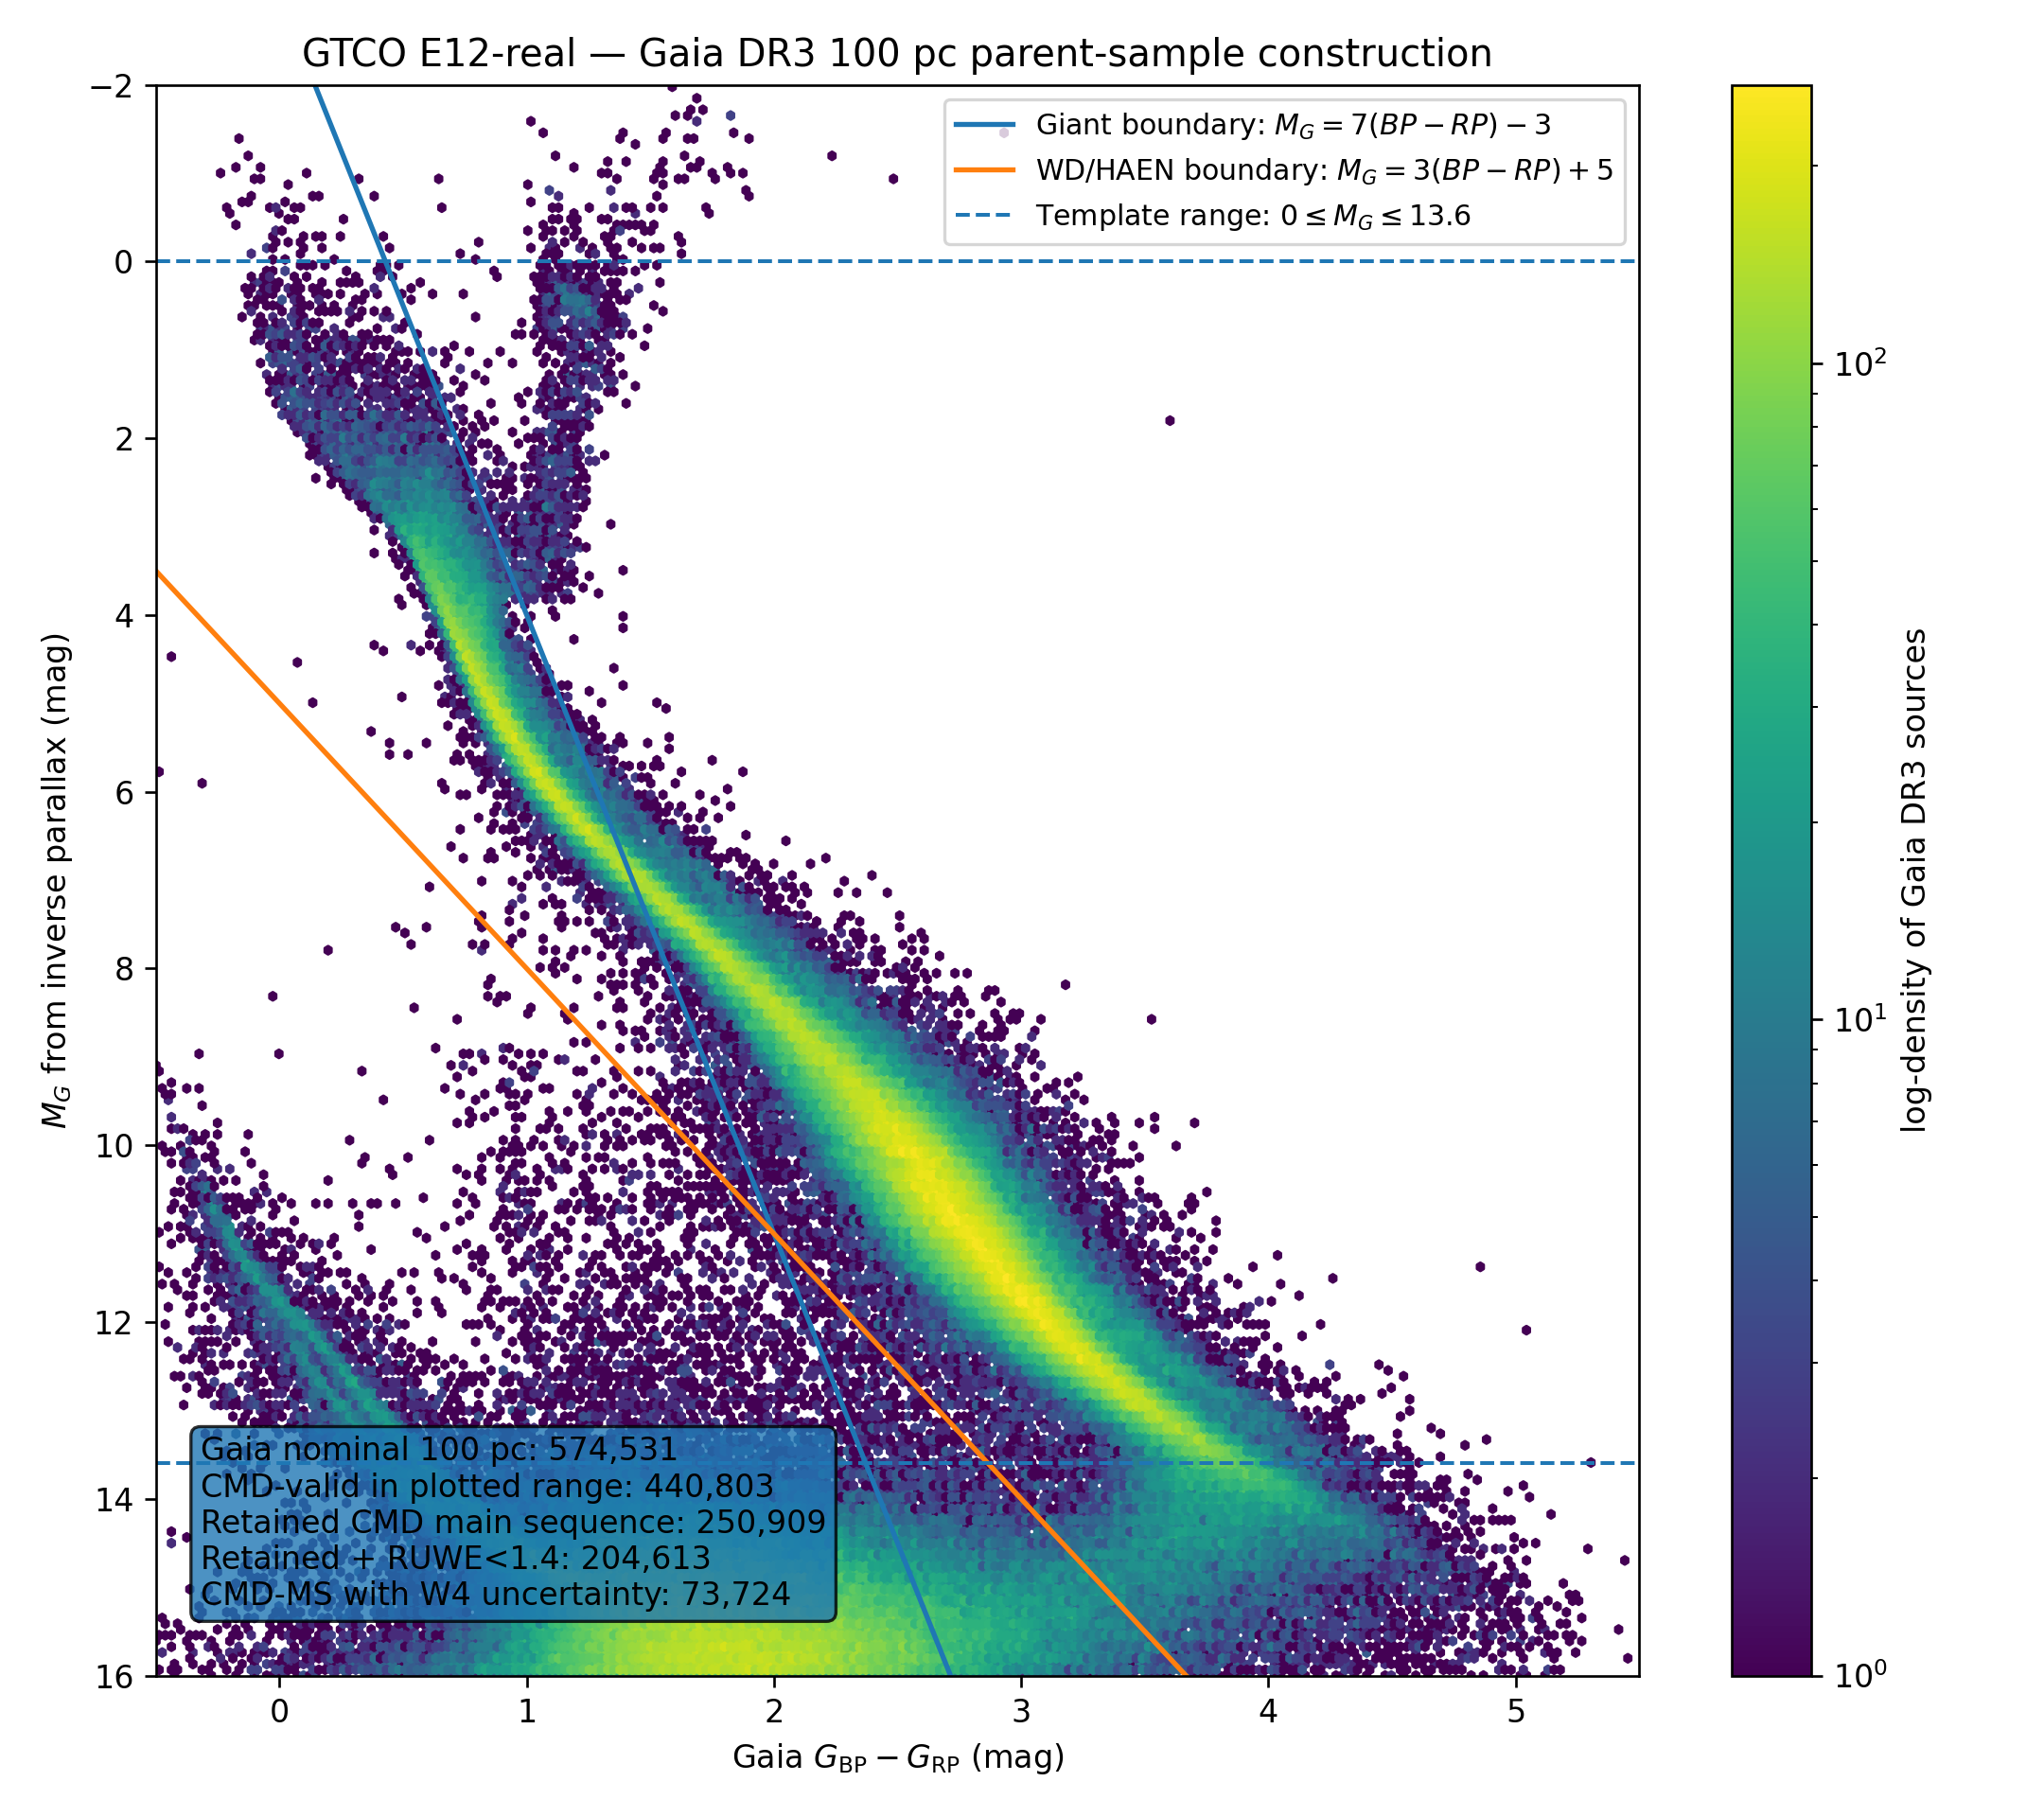
\includegraphics[width=\columnwidth]{figures/fig1_cmd.png}
\caption{Gaia DR3 colour--magnitude selection for the nominal 100-pc parent sample. Downstream host-quality cuts are intentionally not incorporated into this boundary, so their response remains measurable.}
\label{fig:cmd}
\end{figure}

\subsection{Conditioning matters}
\label{sec:conditioning}

The injection experiment described below is not performed on every one of the 250,909 main-sequence stars. It uses a validation-eligible subset with complete baseline photometry and uncertainties. In the real catalogue, 72,716 of the 250,909 CMD-selected stars (28.98 per cent) satisfy the strict ten-band-with-errors requirement used to construct the clean template/validation pool. This fraction is reported to make the conditioning explicit; it is not multiplied into our quoted 0.910 photometric recovery because the strict validation-pool definition is an engineering requirement of the present emulation, not a reconstruction of every admission rule in Hephaistos-II.

We therefore distinguish three different quantities throughout the paper:
\begin{enumerate}
\item a \emph{parent-sample availability} problem, which asks which real stars provide the information needed by a particular analysis;
\item a \emph{conditional injection response}, which asks how a counterfactual Dyson-like source propagates after a usable baseline SED has been established; and
\item an \emph{end-to-end candidate completeness}, which would require all published pipeline stages to be represented by the same executable operator.
\end{enumerate}
Only the second is directly calibrated by the 0.910 recovery reported in Section~\ref{sec:phot}. Table~\ref{tab:semantic} summarizes this distinction.

\begin{table*}
\centering
\caption{Selection terms and their interpretation in this work. ``Measured'' means measured for the stated conditioning set, not necessarily for the full 300-pc Hephaistos-II parent population.}
\label{tab:semantic}
\begin{tabularx}{\textwidth}{p{0.16\textwidth} X p{0.17\textwidth} p{0.25\textwidth}}
\toprule
Term & Operational meaning & Current status & Principal conditioning / limitation\\
\midrule
Baseline catalogue availability & Required real measurements exist & Described, not inverted & Analysis-specific ten-band validation pool\\
$C_{\rm phot\mid V}$ & Injected source survives proxy catalogue cuts and is SED-recognised & Measured & Conditional on validation-eligible hosts $V$\\
$C_{\rm host\mid V}$ & Same validation host passes deterministic Gaia/WISE cuts & Measured & Reconstructed subset of published host cuts\\
$C_{\rm phot\cap host\mid V}$ & Same injected source passes both previous terms & Measured source-by-source & Does not include original CNN/final visual screen\\
$R_{\rm morph}$ & True co-spatial excess remains morphology-acceptable & Measured conditionally & 24 deliberately clean real WISE fields; unsaturated regime\\
$C_{\rm environment}$ & Real field is acceptable before signal injection & Not yet population-calibrated & Requires representative crowded/background sample\\
$C_{\rm linear}$ & Counterfactual remains in usable detector/catalogue regime & Risk surface measured & Saturated images not forward-modelled\\
$C_{\rm DS}$ & Full candidate-operator response & Not yet measured & Requires all stages with matched candidate definition\\
\bottomrule
\end{tabularx}
\end{table*}

\section{Photometric partial-Dyson injection--recovery}
\label{sec:phot}

\subsection{Phenotype model}

We parameterize a partial Dyson sphere by a covering factor $\gamma$ and a waste-heat temperature $T_{\rm DS}$. In the energy-conserving single-temperature model used for the injection library, the observed stellar component is attenuated by $1-\gamma$, while a fraction $\gamma$ of the stellar bolometric flux is thermally re-radiated. The monochromatic model flux density is
\begin{equation}
F_{\nu,{\rm model}}=(1-\gamma)F_{\nu,\star}
+\gamma F_{{\rm bol},\star}
\frac{\pi B_\nu(T_{\rm DS})}{\sigma_{\rm SB}T_{\rm DS}^4}.
\label{eq:dsmodel}
\end{equation}
This is a search phenotype rather than a claim that real technospheres must be blackbodies. The same physical distinction applies to previous Dysonian searches: detectability statements are conditional on the waste-heat phenotype being searched \citep{Wright2014b,Suazo2022}. Our implementation evaluates the model at the adopted band reference wavelengths rather than performing a new full response-curve integration; this and the exact template library are among the reasons we describe the experiment as a close emulation rather than a byte-for-byte reconstruction of Hephaistos-II.

\subsection{Real stellar templates}

The model library is anchored to 265 real stars from the downloaded 100-pc catalogue, mirroring the published number of stellar templates in Hephaistos-II \citep{Suazo2024}. Candidate templates must lie on the CMD main sequence, have RUWE $<1.4$, have all ten magnitudes and the required uncertainty information, satisfy AllWISE ${\tt cc\_flags}=0000$ and ${\tt ext\_flag}=0$, and have a star-only near/mid-infrared baseline residual below 0.2 mag. The final 265 are selected to span the available $M_G$ sequence rather than being a random draw concentrated near the peak of the luminosity function.

Each template is transformed to absolute photometry at 10 pc. For Gaia $G$, $G_{\rm BP}$, and $G_{\rm RP}$, the stellar flux is grey-attenuated by $1-\gamma$. For 2MASS $JHK_s$ and WISE W1--W4, equation~(\ref{eq:dsmodel}) supplies the sum of attenuated stellar light and thermal waste heat. We combine the 265 templates with 49 temperatures between 100 and 700 K and 17 covering factors between 0.1 and 0.9, producing
\begin{equation}
265\times49\times17=220,745
\end{equation}
model SEDs. The published Hephaistos-II description provides the ranges and model counts; because the exact internal grid spacing was not available to this reconstruction, we use uniform grids within those ranges.

\subsection{Independent validation stars and noise model}

A separate set of 3,000 real main-sequence stars is excluded from the 265-template library and used for validation. These stars have all ten bands and their required errors available, baseline stellar-model residual below 0.2 mag, and a conservative star-only mid-infrared residual proxy below 0.5 mag. The validation stars are sampled across the sorted $M_G$ sequence to maintain broad coverage of the selected main sequence rather than selecting 3,000 adjacent objects in luminosity.

The truth grid contains nine waste-heat temperatures,
\begin{equation}
T_{\rm DS}=\{100,150,200,250,300,400,500,600,700\}\ {\rm K},
\end{equation}
and six covering factors,
\begin{equation}
\gamma=\{0.1,0.2,0.3,0.5,0.7,0.9\},
\end{equation}
for 54 truth cells. For each source, the counterfactual flux is perturbed using that source's measured per-band photometric uncertainty in flux space. The noisy ten-band SED is transformed to absolute magnitudes and queried against the 220,745-model library by Euclidean nearest-neighbour distance. Following the unweighted magnitude-space criterion described for Hephaistos-II, the recognition statistic is
\begin{equation}
{\rm RMSE}=\frac{d_{10}}{\sqrt{10}},
\end{equation}
with acceptance at RMSE $\le0.2$ mag \citep{Suazo2024}. The use of an unweighted magnitude RMSE prevents the highest signal-to-noise optical bands from automatically dominating the W3/W4 excess geometry, but it is also a deliberate model choice and is not interpreted as a likelihood.

\subsection{Catalogue-survival proxy and saturation flag}

Before model recognition, an injected source must retain positive noisy flux in all ten bands, have injected Gaia $G\le21$, have expected 2MASS $JHK_s$ signal-to-noise ratio $>2$, and have expected W3/W4 signal-to-noise ratio $>3.5$. These cuts are a reconstruction of the relevant photometric stage, not the complete Hephaistos-II candidate operator. WISE saturation risk is tracked separately. We use the WISE characteristic point-source saturation magnitudes W3 $=3.8$ and W4 $=-0.4$ mag, at which approximately half of catalogue sources show saturation; saturated-source photometry can remain recoverable from unsaturated wings, but its accuracy becomes progressively less reliable \citep{Cutri2012}.

Across the 54 truth cells, the mean catalogue-survival proxy is 0.9863. Conditional on catalogue survival, the mean model-recognition probability is 0.9206. Counting both survival and recognition, the arithmetic mean over the 54 equally weighted truth cells is
\begin{equation}
\left\langle C_{\rm phot\mid V}\right\rangle=0.9101.
\end{equation}
This is a grid average, not a population-marginalized completeness: changing the phenotype distribution over $(T_{\rm DS},\gamma)$ would change the average. Figure~\ref{fig:photrec} shows the response surface. The weakest cell is the cold, high-covering-factor region, where catalogue survival, finite-band contrast, and saturation become most consequential.

\begin{figure}
\centering
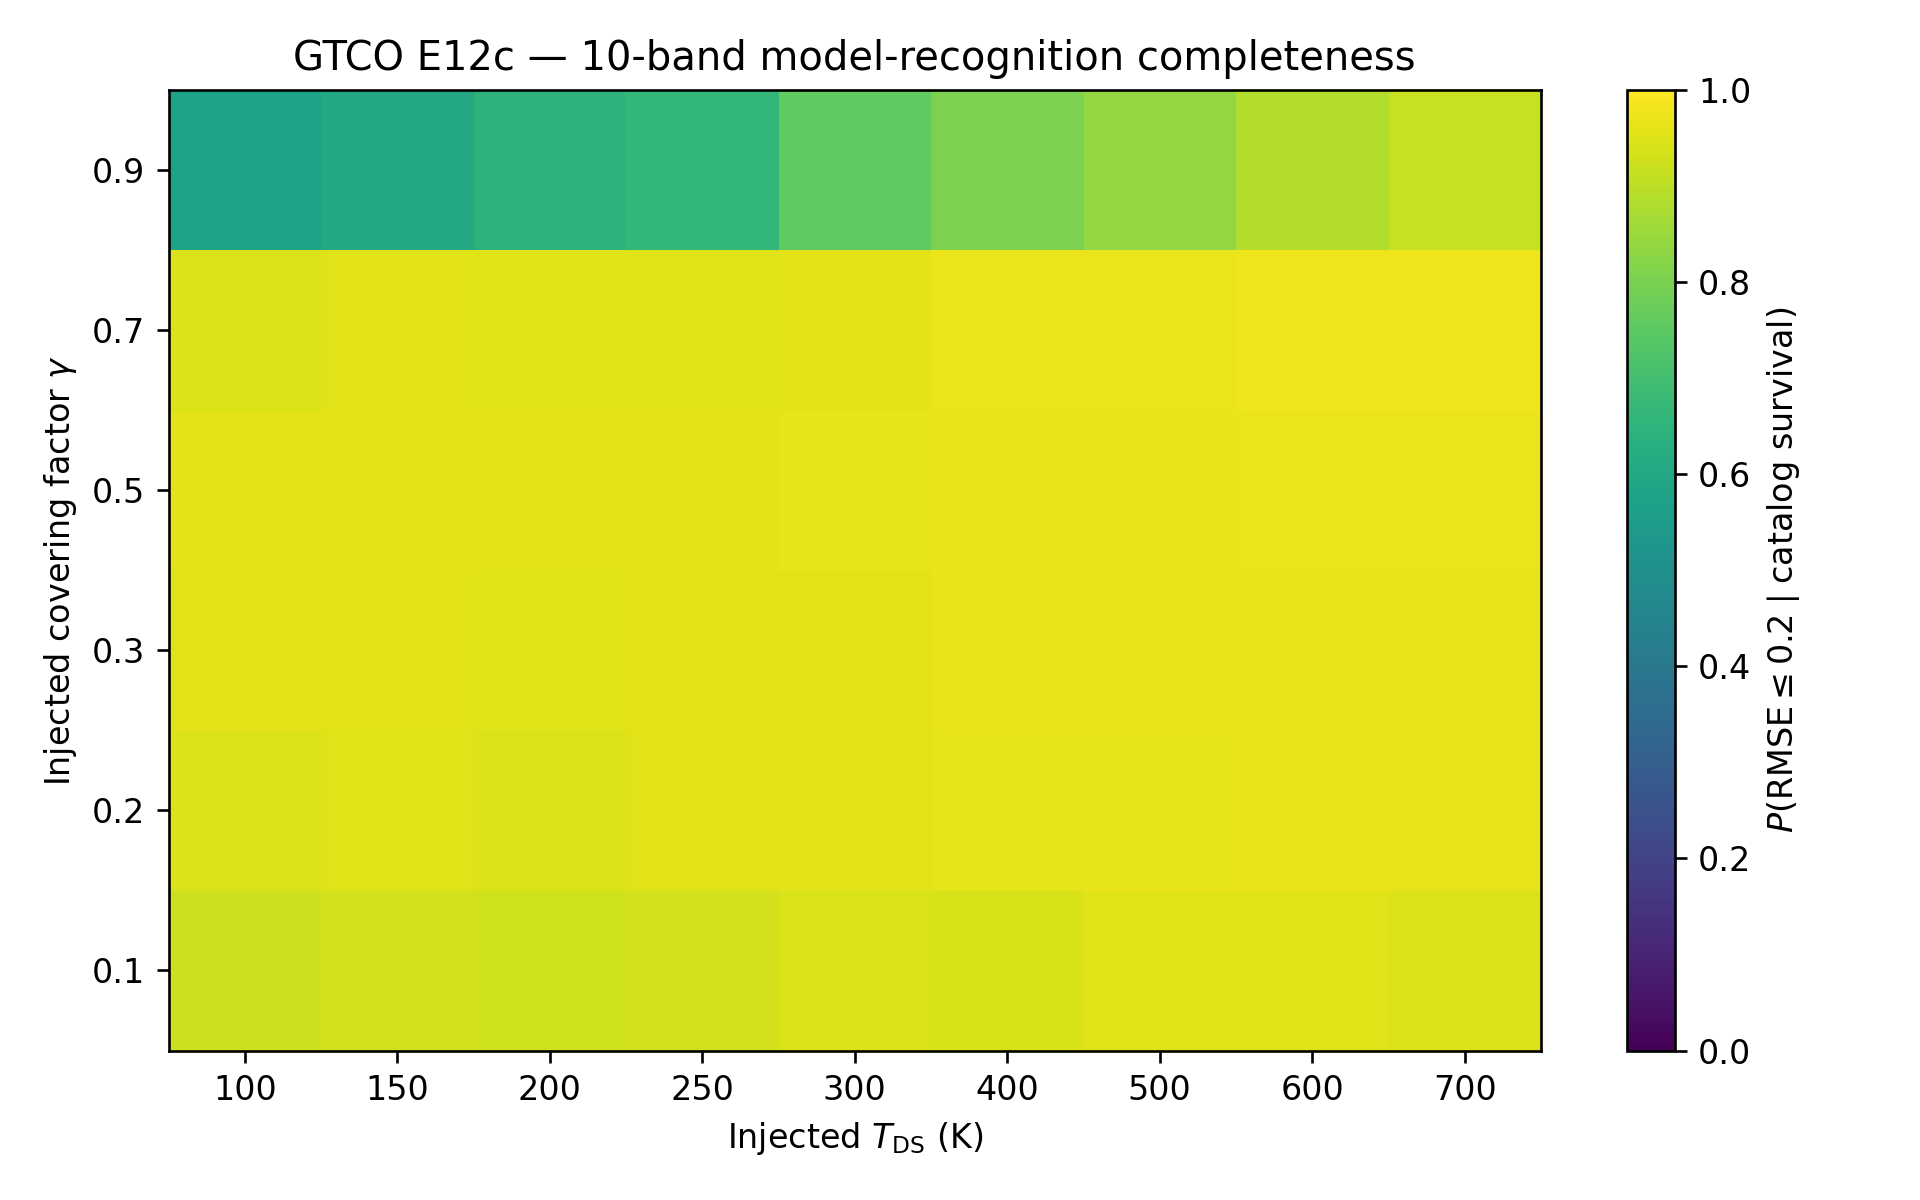
\includegraphics[width=\columnwidth]{figures/fig2_photometric_recovery.png}
\caption{Real-catalogue injection--recovery across the 54-cell partial-Dyson truth grid. The response includes the stated catalogue-survival proxy and ten-band model recognition, conditional on the validation-eligible real stellar sample. It is not the end-to-end candidate completeness.}
\label{fig:photrec}
\end{figure}

\subsection{Independent reconstruction audit}

Before submission, the 220,745-model library and 54-cell validation experiment were independently rebuilt from frozen input tables. The reconstructed mean catalogue survival is 0.986309, compared with 0.986259 in the earlier frozen analysis. The reconstructed mean photometric recovery is 0.910543, compared with 0.910074, an absolute difference of $4.7\times10^{-4}$. The source-level reconstruction is therefore used for the joint host-selection experiment below.

\section{Deterministic host selection}
\label{sec:hostcuts}

\subsection{Gaia/WISE fields and operational cuts}

Hephaistos-II applies astrophysical and catalogue-quality filters intended to reduce stellar activity, variability, astrometric complexity, source extension, and non-stellar contamination \citep{Suazo2024}. We downloaded the Gaia DR3 quantities needed to reconstruct the available cuts, including H$\alpha$ equivalent width and uncertainty, $G$-band observation counts and flux-over-error, and the DSC combined probability of being a single star. Gaia DR3 Apsis provides the H$\alpha$ and classification products used here \citep{Creevey2023}. RUWE is the Gaia renormalised astrometric goodness-of-fit statistic \citep{Lindegren2021}; it is itself known to define a non-trivial Gaia subset selection \citep{EverallBoubert2022}.

Our operational host gate requires
\begin{align}
EW_{{\rm H}\alpha}+3\sigma_{EW}&\ge0,\\
G_{\rm var}&\le2,\\
{\rm RUWE}&\le1.4,\\
{\tt ext\_flag}&=0,\\
P_{\rm Gaia,star}&>0.9.
\end{align}
The H$\alpha$ condition rejects a source only when the measured equivalent width plus three standard deviations remains on the emission side of the adopted sign convention. Missing H$\alpha$ does not by itself constitute evidence for emission and therefore does not trigger this rejection. In contrast, missing RUWE, WISE extension flag, stellar-classification probability, or variability statistic cannot satisfy their positive quality requirements and are treated as failures of those individual cuts. These semantics are frozen in the public reproduction script.

\subsection{Variability statistic and sensitivity to the reference window}

We reconstruct the reported $G$-band variability statistic from
\begin{equation}
\nu_G=\frac{\sqrt{N_{{\rm obs},G}}}
{{\tt phot\_g\_mean\_flux\_over\_error}},
\end{equation}
and normalize it by a local median among sources of similar $G$ magnitude,
\begin{equation}
G_{\rm var}=\frac{\nu_G}
{\operatorname{median}_{\rm similar\,G}(\nu_G)}.
\end{equation}
The published description does not uniquely specify the numerical width of the ``similar-flux'' neighbourhood. We therefore evaluated rolling reference windows of 500, 1,000, and 5,000 magnitude-sorted sources. In the 250,909-star CMD main-sequence sample, the full host-pass fractions are 0.522819, 0.522875, and 0.522994, respectively. Pairwise classification disagreement is below 0.4 per cent. We adopt 1,000 as the default while carrying the window sensitivity as an audit rather than presenting the choice as known exactly.

\subsection{Host response in the injection validation sample}

The scientifically relevant host term for combining with Section~\ref{sec:phot} is the host response of the same individual 3,000 validation stars. Sequential retention is 0.925 after H$\alpha$, 0.760 after adding $G_{\rm var}$, 0.572 after RUWE, 0.526 after AllWISE extension, and
\begin{equation}
C_{\rm host\mid V}=0.442
\end{equation}
after the stellar-classification requirement.

Because the five cuts overlap, the marginal number removed by a cut depends on its order. We therefore calculated a Shapley attribution over all $5!=120$ cut orderings. RUWE accounts for 38.9 per cent of the attributed host-selection loss, followed by $G_{\rm var}$ (20.6 per cent), stellar-classification probability (20.3 per cent), WISE extension (11.6 per cent), and H$\alpha$ (8.6 per cent; Fig.~\ref{fig:shapley}). This is a decomposition of selection burden, not an argument that the largest-contribution cut is astrophysically unjustified.

\begin{figure}
\centering
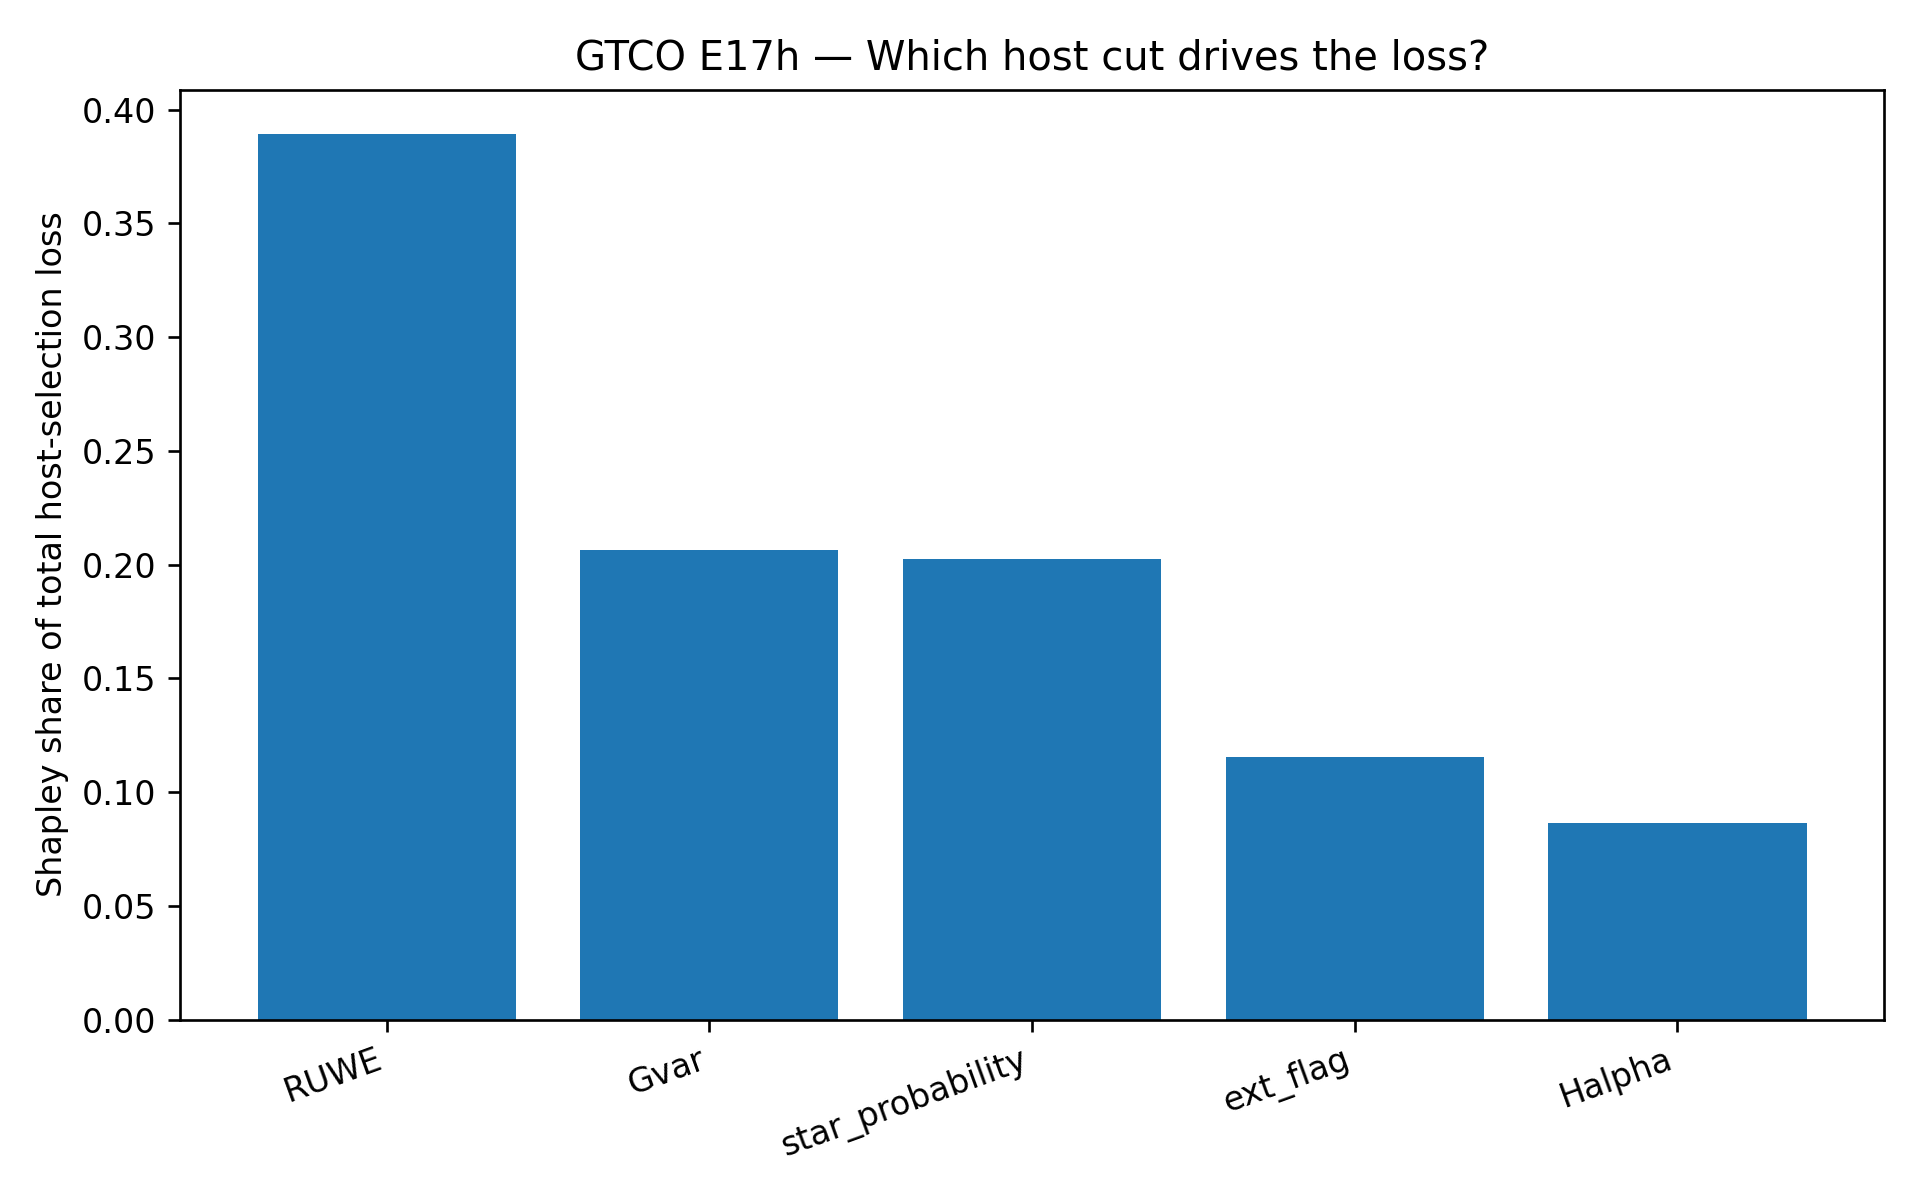
\includegraphics[width=\columnwidth]{figures/fig4_hostcut_shapley.png}
\caption{Shapley attribution of the overlapping host-selection loss in the 3,000-star validation sample. The value measures how strongly each cut contributes to removal across all cut orderings; it does not evaluate whether the cut should be retained.}
\label{fig:shapley}
\end{figure}

\subsection{Source-level joint photometric and host selection}
\label{sec:joint}

A common completeness approximation is to multiply stage-averaged responses,
\begin{equation}
C_{\rm joint}\stackrel{?}{=}
\langle C_{\rm phot}\rangle\langle C_{\rm host}\rangle.
\end{equation}
This equality is exact only under an appropriate independence condition. Here the two stages share dependencies on real source properties: brightness, colour, astrometric quality, classification confidence, and catalogue measurement quality are not generated independently.

We therefore apply the host gate to the same source identities used in each injection. Averaged over the 54 truth cells,
\begin{equation}
\left\langle C_{\rm phot\cap host\mid V}\right\rangle=0.4142,
\end{equation}
whereas the product of stage means gives
\begin{equation}
0.91054\times0.442=0.4025.
\end{equation}
The source-level response is about 0.0118 higher in absolute terms, or 2.9 per cent higher relative to the factorised approximation. Figure~\ref{fig:hostsurface} shows the response as a function of injected phenotype.

\begin{figure}
\centering
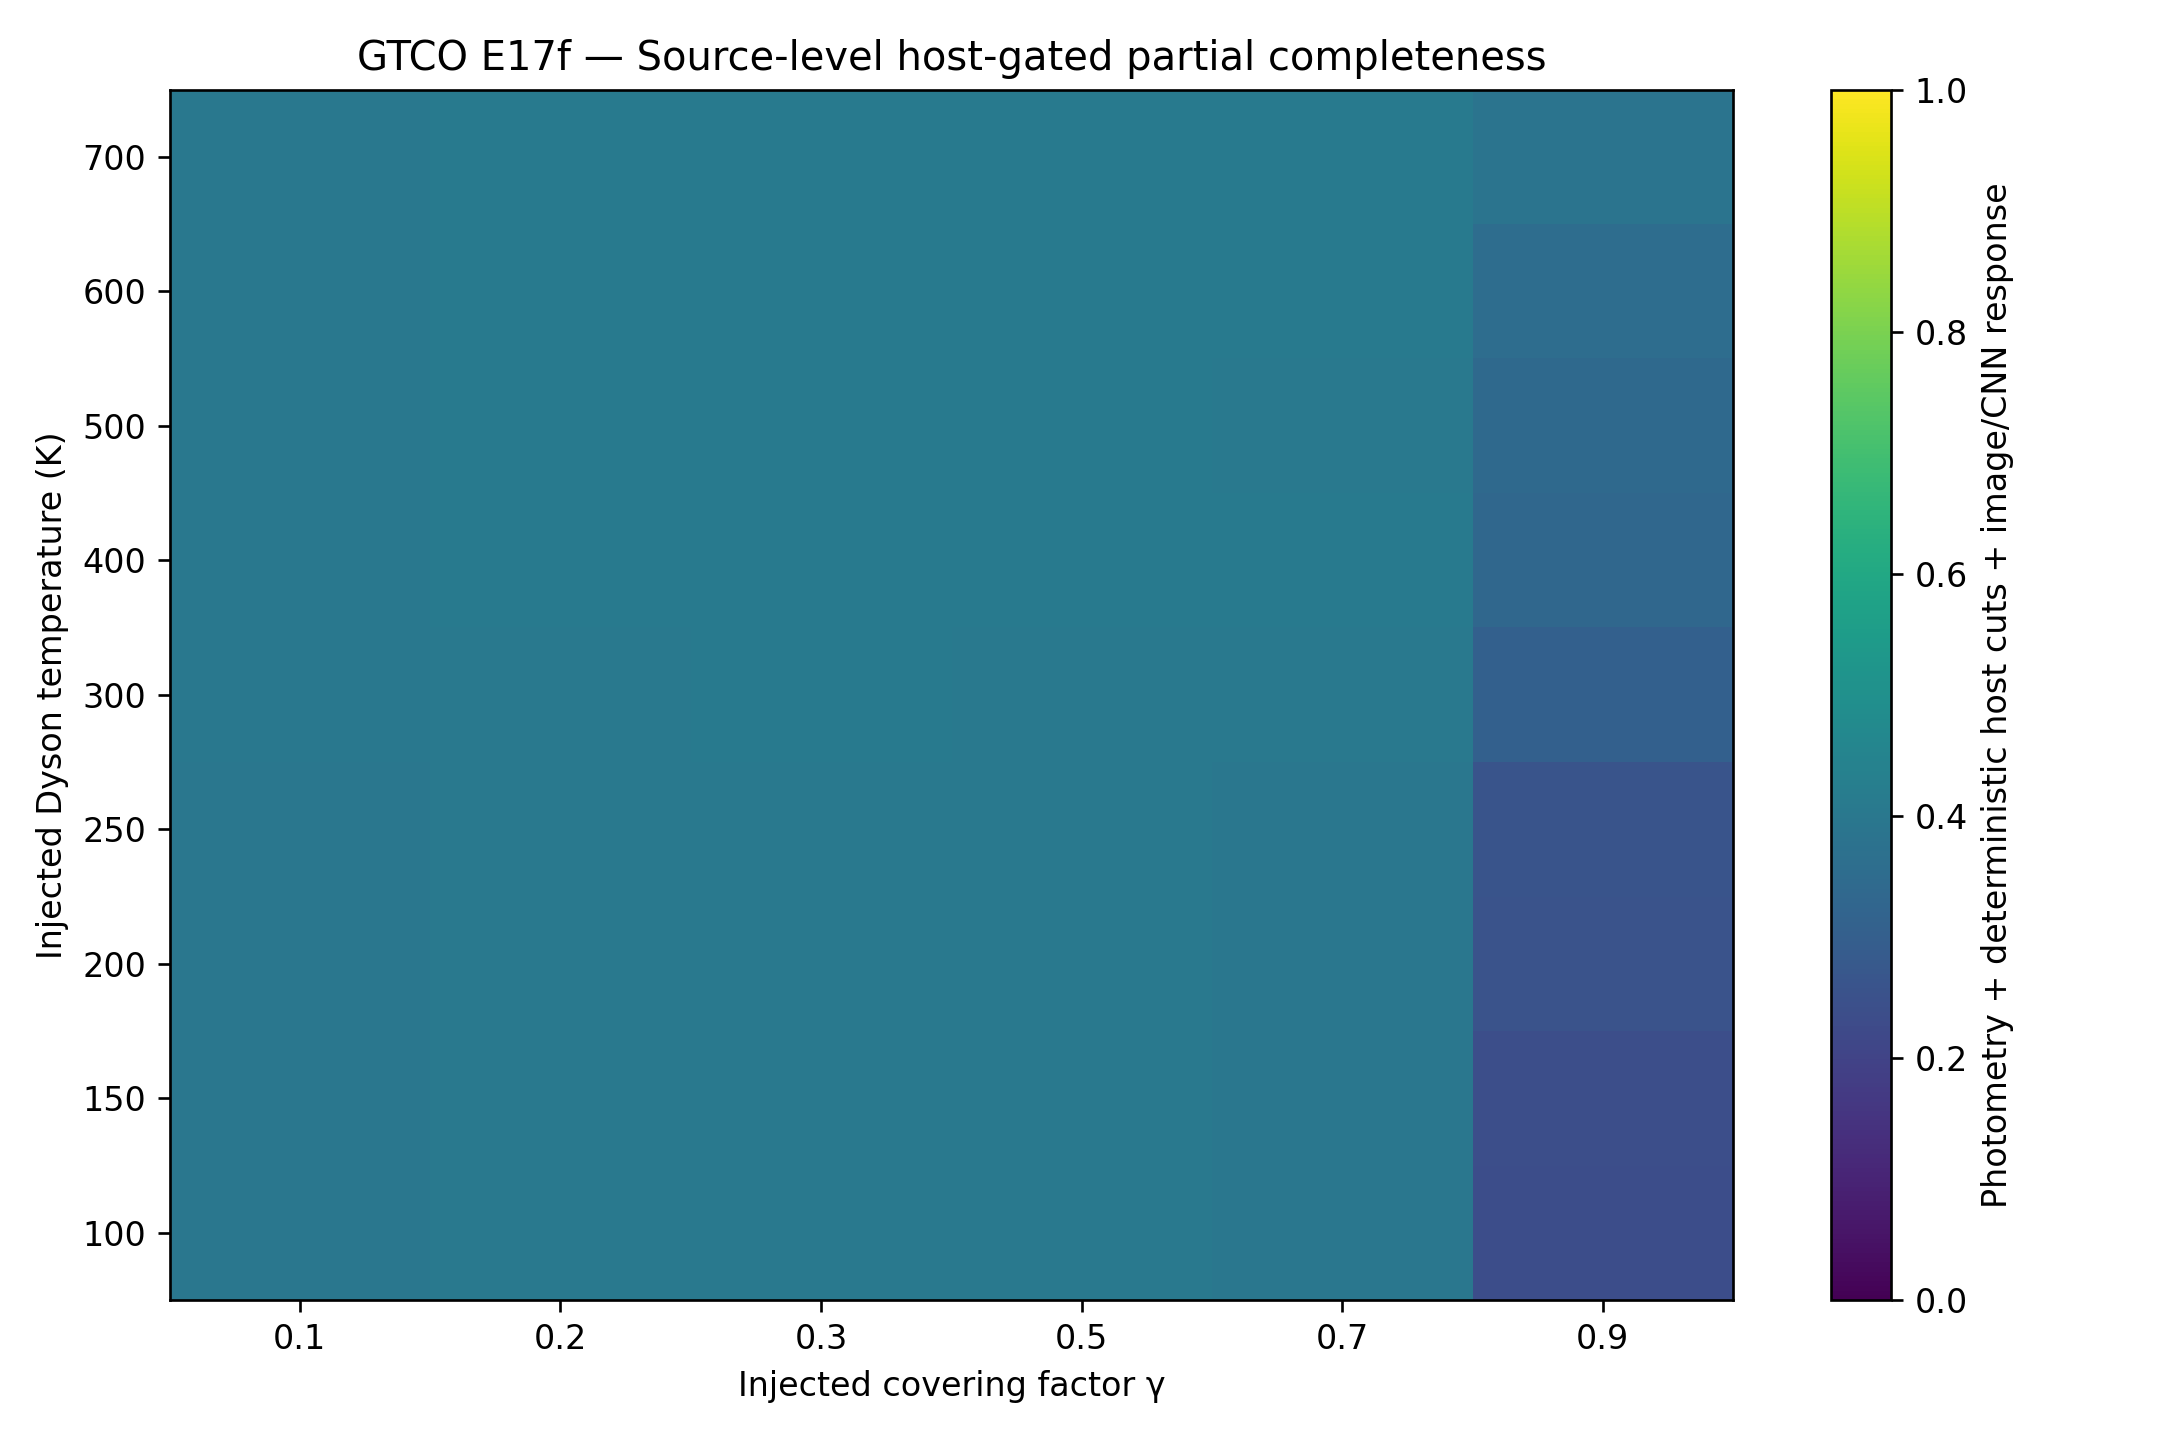
\includegraphics[width=\columnwidth]{figures/fig3_host_gated_completeness.png}
\caption{Source-level joint photometric and deterministic host-selection response across the partial-Dyson grid. Each injection is combined with the host quality of the same real validation star; the surface is not produced by multiplying two global stage means.}
\label{fig:hostsurface}
\end{figure}

This difference is not large enough to dominate the present error budget, but it demonstrates a general principle for end-to-end technosignature completeness:
\begin{equation}
E[C_1(\mathbf{x})C_2(\mathbf{x})]
\ne
E[C_1(\mathbf{x})]E[C_2(\mathbf{x})]
\end{equation}
when the stages share source-property dependence. For rare-event population inference, source-level signal injection is therefore preferable to multiplying stage efficiencies whenever the data permit it.

\section{Real AllWISE image injection}
\label{sec:image}

\subsection{AllWISE image products}

The image experiment uses 24 bright, low-confusion calibration stars from the 3,000-star validation set. All 24 have AllWISE ${\tt cc\_flags}=0000$, ${\tt ext\_flag}=0$, and Gaia RUWE $<1.4$; 23/24 have zero reported WISE mates and a Gaia--AllWISE catalogue offset below 0.3 arcsec, while one retained boundary case has one reported mate and an offset of 0.446 arcsec. The sample spans W3 $=4.46$--8.48 mag. For each star we retrieved W3 and W4 AllWISE Atlas intensity, uncertainty, and depth-of-coverage cutouts, giving
\begin{equation}
24\times2\times3=144
\end{equation}
FITS products. The AllWISE Atlas has a pixel scale of 1.375 arcsec pixel$^{-1}$ and supplies co-registered intensity, uncertainty, and coverage products in each WISE band \citep{Cutri2013}. These fields are an image-calibration sample, not a representative draw from the full distribution of WISE backgrounds, crowding, and source brightness. This design is deliberate: the experiment asks whether adding a true co-spatial point-source excess to an otherwise acceptable image tends to create a morphology rejection.

The AllWISE documentation notes that resampling and interpolation produce correlated pixel noise in Atlas images \citep{Cutri2013}. Consequently, the uncertainty-weighted residual statistic used below is treated as a \emph{pseudo}-$\chi^2$ morphology feature rather than a formally calibrated independent-pixel goodness-of-fit probability. We test the dependence of our result on this feature explicitly in Section~\ref{sec:image_robustness}.

\subsection{Epoch-consistent source centring}

Gaia astrometric positions are referenced to J2016.0 \citep{Lindegren2021}, whereas W3/W4 AllWISE coadds are dominated by the WISE cryogenic epoch near 2010. We propagate each Gaia position to 2010.5 using its Gaia proper motion before locating the stellar position in the WISE WCS. Across the 24 image-calibration stars, the median 2016.0-to-2010.5 displacement is 0.479 arcsec, the 95th percentile is 1.43 arcsec, and the maximum is 2.81 arcsec. Such shifts are non-negligible compared with the 1.375 arcsec Atlas pixels and would be especially problematic when centroid offset is itself used as a morphology diagnostic. Recent archival analyses of Hephaistos candidates similarly propagate Gaia positions to the WISE epoch before comparing astrometry with mid-infrared centroids \citep{Ren2026}.

\subsection{Empirical PSF and open morphology statistic}

For each band, real source-centred cutouts are background-subtracted in an outer annulus, aligned at sub-pixel precision using their positive central flux, normalized by a central aperture, and combined into an empirical point-source template. The final submission analysis is leave-one-host-out (LOHO): when star $i$ is tested, the empirical PSF is rebuilt from the other 23 stars only.

For a test image, the empirical PSF amplitude is estimated by uncertainty weighting over a central fitting region. The open morphology feature vector contains
\begin{enumerate}
\item the logarithm of an uncertainty-weighted residual pseudo-$\chi^2$;
\item the logarithm of the summed absolute residual normalized by fitted point-source amplitude;
\item the positive-flux centroid offset from the propagated stellar position; and
\item the logarithm of the second-moment major/minor axis ratio.
\end{enumerate}
For each held-out star, the 23 non-test hosts also define the robust feature centre and scale using the median and median absolute deviation. The anomaly score is the maximum robust standardized deviation among the active features. Our default empirical envelope sets the threshold to the maximum score among the 23 training hosts. Thus a held-out baseline image is called clean only if it lies within the entire non-test empirical envelope. This has finite-sample granularity of order one host in 24; it is a transparent open operator, not a reconstruction of the proprietary state of the original Hephaistos image CNN.

\subsection{Co-spatial waste-heat injection and linearity domain}

For each held-out real image, we scan
\begin{equation}
T_{\rm DS}=\{100,150,200,250,300\}\ {\rm K}
\end{equation}
and
\begin{equation}
\gamma=\{0.03,0.05,0.08,0.10,0.14,0.16\},
\end{equation}
producing 720 counterfactuals per band. The physical flux ratio between the baseline catalogued W3/W4 source and the counterfactual follows equation~(\ref{eq:dsmodel}). That ratio is converted to an incremental image amplitude by scaling the fitted point-source amplitude of the real field. The injected image is therefore
\begin{equation}
I_{\rm inj}(x,y)=I_{\rm real}(x,y)+\Delta A\,P_{-i}(x,y),
\end{equation}
where $P_{-i}$ is the empirical PSF constructed without the test host. This formulation preserves the real background, neighbours, coverage, and pixel noise while testing the effect of adding a co-spatial point-like MIR component.

The image operation assumes an approximately linear response. Counterfactuals brighter than the characteristic WISE saturation onsets W3 $=3.8$ mag or W4 $=-0.4$ mag are therefore flagged and excluded from the linear morphology-retention statement \citep{Cutri2012}. Within this deliberately selected 24-star sample and the low-$\gamma$ image grid, 49.7 per cent of W3 counterfactuals and 13.1 per cent of W4 counterfactuals cross those characteristic thresholds. These are not population saturation rates; they are diagnostics of the chosen bright host sample and phenotype grid. WISE can still extract some saturated-source photometry from unsaturated PSF wings, so a full $C_{\rm linear}$ calculation would require explicit bright-source/non-linear forward modelling rather than treating these thresholds as hard catalogue incompleteness.

\section{Real-image results and robustness}
\label{sec:image_results}

\subsection{Leave-one-host-out conditional retention}

In W3, 23 of the 24 held-out baseline fields lie within their corresponding LOHO empirical envelope. After excluding saturated counterfactuals, these 23 independent baseline-clean hosts contribute 332 valid injected grid cases. No valid injection is rejected. W4 likewise has 23 independent baseline-clean hosts and 596 valid unsaturated injections, with no rejection.

The repeated $(T_{\rm DS},\gamma)$ grid cells are not statistically independent realizations of the image environment. We therefore define a host-level success as a host for which all of its valid injected phenotypes remain accepted. This yields 23/23 successful independent hosts in W3 and 23/23 in W4. Using the exact binomial interval of \citet{ClopperPearson1934}, the one-sided 95 per cent lower confidence limit is
\begin{equation}
R_{\rm morph,W3}>0.878,
\end{equation}
and identically
\begin{equation}
R_{\rm morph,W4}>0.878.
\end{equation}
For a joint W3+W4 requirement, 22 independent hosts have at least one grid cell that is baseline-clean and unsaturated in both bands. All 22 pass all valid paired injections, giving
\begin{equation}
R_{\rm morph,W3\cap W4}>0.873
\end{equation}
at one-sided 95 per cent confidence. These intervals use the host, not the repeated $(T_{\rm DS},\gamma)$ grid cell, as the independent Bernoulli unit. The zero observed failures therefore do not imply unit retention with negligible uncertainty: with only 23 (22 joint) independent hosts, the finite-sample lower bounds remain materially below unity. This host-level interpretation is used throughout the paper. Figure~\ref{fig:imageretention} shows the host-level result and its finite-sample lower limits.

\begin{figure}
\centering
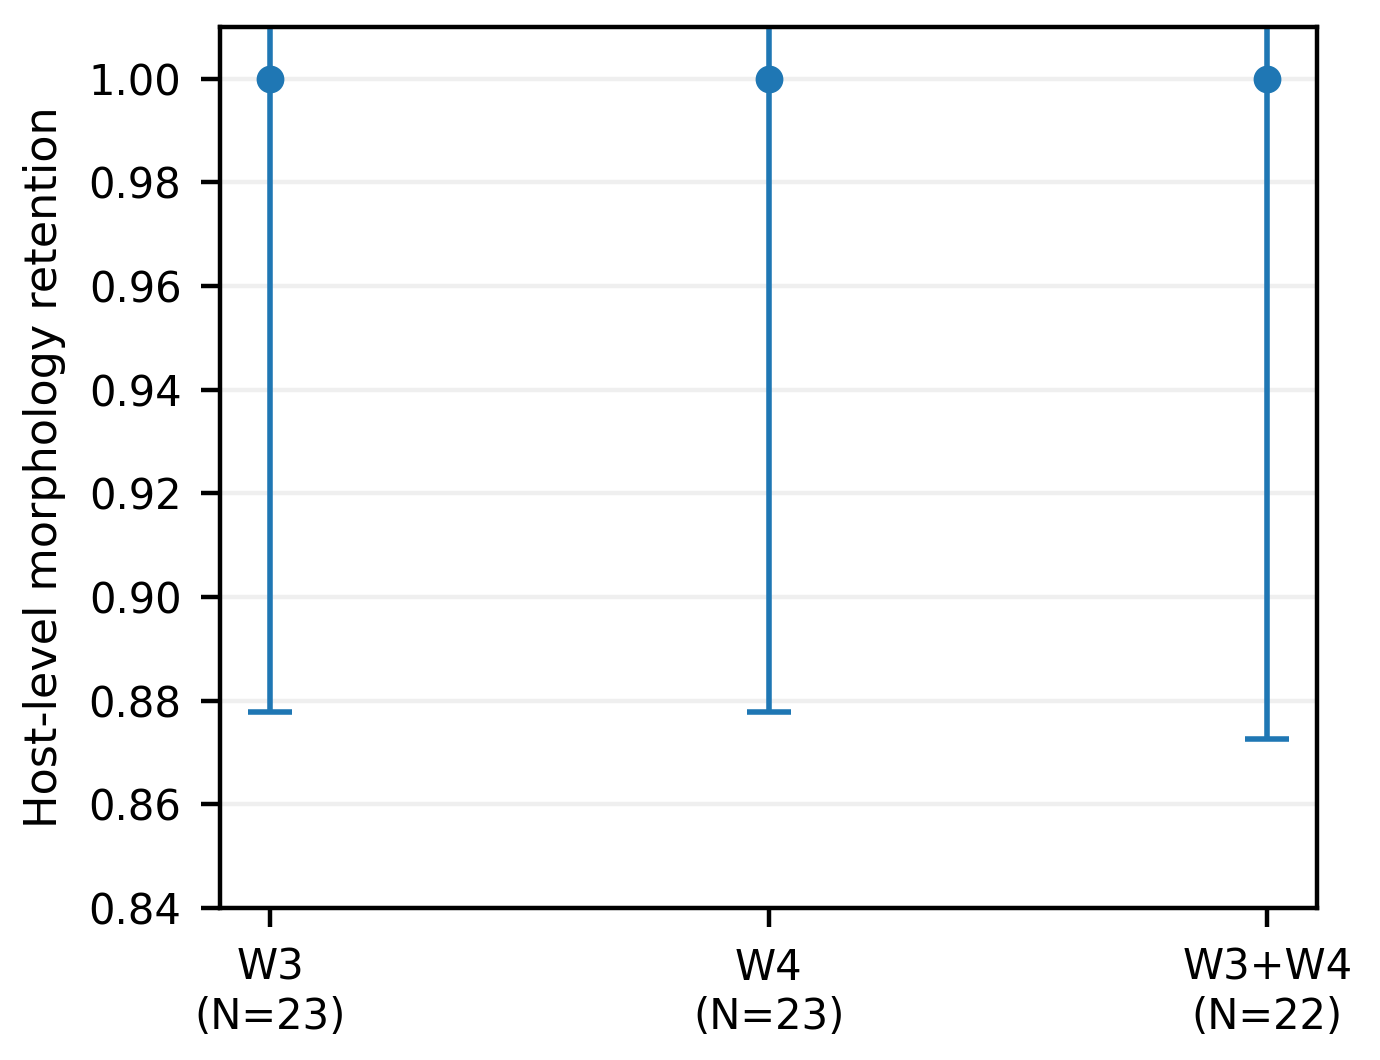
\includegraphics[width=\columnwidth]{figures/fig5_loho_host_retention.png}
\caption{Leave-one-host-out real-image morphology retention. Points show the observed host-level success fraction and error bars extend to the one-sided 95 per cent exact lower bound. The independent unit is the real host, not the repeated injection grid cell.}
\label{fig:imageretention}
\end{figure}

The injected excess usually moves the open morphology statistic toward, rather than away from, the point-source locus. Among valid LOHO injections, 76.8 per cent of W3 grid cases and 85.9 per cent of W4 grid cases have a negative anomaly-score change. The median score changes are $-0.539$ and $-0.503$, respectively. Figure~\ref{fig:scorechange} shows the full valid counterfactual distribution. The horizontal zero-score-change ridge contains cases for which the active maximum standardized feature is unchanged even though another component of the morphology vector improves.

\begin{figure}
\centering
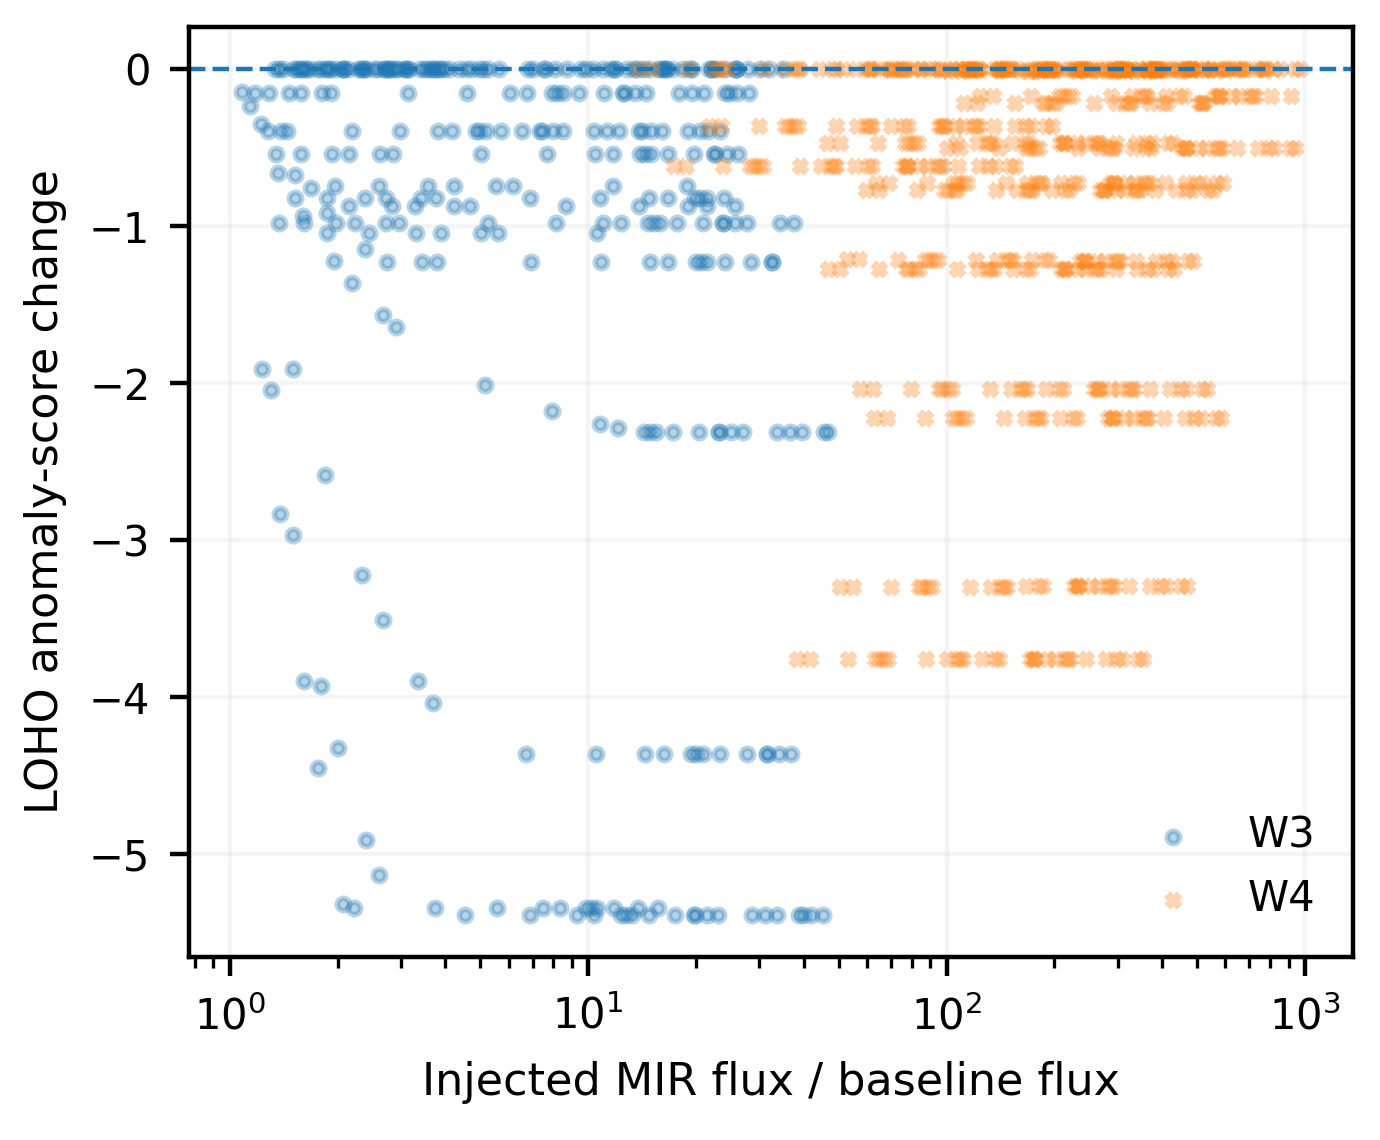
\includegraphics[width=\columnwidth]{figures/fig6_loho_score_change.png}
\caption{Change in the leave-one-host-out morphology anomaly score after co-spatial waste-heat injection, restricted to baseline-clean and unsaturated counterfactuals. Negative values mean that the image moves toward the empirical point-source locus under the open morphology statistic.}
\label{fig:scorechange}
\end{figure}

\subsection{Metric and threshold ablation}
\label{sec:image_robustness}

The AllWISE Atlas uncertainty map does not encode the full inter-pixel covariance introduced by coaddition, so the pseudo-$\chi^2$ feature should not be essential to the scientific conclusion. We reran the complete LOHO experiment using four feature sets: the default four-metric score; the same score with pseudo-$\chi^2$ removed; centroid plus axis ratio only; and normalized residual only. We also changed the empirical envelope from the maximum training score to the 95th and 90th percentiles of the 23 training-host scores. Table~\ref{tab:ablation} summarizes the result.

\begin{table*}
\centering
\caption{LOHO image-response robustness. $N_{\rm clean}$ is the number of held-out baseline hosts satisfying the specified empirical envelope. $N_{\rm inj}$ counts valid unsaturated injections across those hosts. Every listed configuration retains all valid injections; the changing $N_{\rm clean}$ reflects the stricter baseline envelope, not signal-induced image failures.}
\label{tab:ablation}
\begin{tabular}{lllrrr}
\toprule
Band & Feature set & Training-envelope threshold & $N_{\rm clean}$ & $N_{\rm inj}$ & Injection retention\\
\midrule
W3 & four metrics & 90th percentile & 20 & 288 & 1.000\\
W3 & four metrics & 95th percentile & 22 & 316 & 1.000\\
W3 & four metrics & maximum & 23 & 332 & 1.000\\
W3 & no pseudo-$\chi^2$ & maximum & 23 & 332 & 1.000\\
W3 & centroid + axis ratio & maximum & 23 & 332 & 1.000\\
W3 & normalized residual only & maximum & 23 & 332 & 1.000\\
\addlinespace
W4 & four metrics & 90th percentile & 21 & 563 & 1.000\\
W4 & four metrics & 95th percentile & 22 & 593 & 1.000\\
W4 & four metrics & maximum & 23 & 596 & 1.000\\
W4 & no pseudo-$\chi^2$ & maximum & 23 & 596 & 1.000\\
W4 & centroid + axis ratio & maximum & 23 & 596 & 1.000\\
W4 & normalized residual only & maximum & 23 & 596 & 1.000\\
\bottomrule
\end{tabular}
\end{table*}

The conditional retention result therefore does not depend on treating the uncertainty map as an independent-pixel covariance model and persists under stricter baseline morphology envelopes. The experiment supports a narrow physical statement: adding a co-spatial point-source excess to a field that already looks point-like does not, in the tested regime, naturally create the morphology of an offset blend or extended contaminant.

\subsection{Image-stage decomposition}

The result motivates separating three conceptually different probabilities:
\begin{equation}
C_{\rm image}
=C_{\rm environment}\,C_{\rm linear}\,R_{\rm morph}.
\label{eq:image_decomp}
\end{equation}
$C_{\rm environment}$ is the probability that the underlying real field is acceptable before technosignature injection, given crowding, background structure, artefacts, and line-of-sight objects. $C_{\rm linear}$ is the probability that the counterfactual remains in a detector/catalogue regime for which the adopted image and photometry operators are valid. $R_{\rm morph}$ is the probability that a true co-spatial signal remains morphology-acceptable conditional on the first two requirements. The current real-image experiment constrains $R_{\rm morph}$ on a deliberately clean calibration set. It does not measure $C_{\rm environment}$ for the survey population.

This distinction is observationally consequential. WISE confusion is a known failure mode in ordinary infrared-excess surveys \citep{KennedyWyatt2012}, and the Hephaistos follow-up sequence now provides direct examples in which higher angular resolution identifies background galaxies that are unresolved or blended in WISE \citep{Ren2025,Ren2026,Zackrisson2026}. A future representative field sample should therefore target $C_{\rm environment}$ rather than interpreting the present 23/23 result as $C_{\rm image}=1$.

\section{From candidates to population constraints}
\label{sec:population}

Equation~(\ref{eq:selection_inversion}) becomes useful only after every factor has a matched operational definition. The seven final candidates reported by \citet{Suazo2024}, for example, provide a final-candidate rate for the published Hephaistos-II decision chain. Our 0.910 photometric response is not the completeness of that seven-candidate operator: it does not reproduce the original CNN weights, the full image-confusion decision, every downstream astrophysical cut, or the final manual review. Dividing the published final-candidate rate by 0.910 would therefore combine incompatible selection definitions.

Likewise, $C_{\rm DS}$ is not a universal scalar. Let $\boldsymbol\psi$ denote technosignature phenotype parameters such as $(T_{\rm DS},\gamma)$ and let $\mathbf{x}$ denote host and observing conditions. A population-averaged completeness is
\begin{equation}
\bar C_{\rm DS}=
\int C_{\rm DS}(\boldsymbol\psi,\mathbf{x})
\,p(\boldsymbol\psi,\mathbf{x}\mid{\rm DS})
\,{\rm d}\boldsymbol\psi\,{\rm d}\mathbf{x}.
\label{eq:marginal_completeness}
\end{equation}
The numerical value therefore depends on a declared phenotype distribution, or else should be reported as a response surface rather than compressed into one number. This is why the arithmetic mean of 0.910 over our 54 equally weighted truth cells is useful as an experiment summary but should not be inserted uncritically into an occurrence estimate.

The same logic applies to candidate composition. $\pi_{\rm DS}$ is the fraction of objects admitted by the candidate operator that genuinely belong to the target phenotype. It is not obtained by normalizing a discriminative SED score unless that score has been calibrated as a likelihood for the selected population. High-resolution follow-up changes what is known about individual candidates and, with an explicitly modelled follow-up selection, can improve inference on candidate composition; it does not retroactively convert an unmatched upstream completeness into a final-pipeline response.

The immediate population-inference target is therefore a selection-consistent chain in which the parent definition, candidate definition, signal injection, image/environment response, and follow-up interpretation are frozen together. The current work calibrates several of those pieces and, equally importantly, identifies the unmeasured terms instead of absorbing them into an apparently precise scalar.

\section{Discussion}

\subsection{Relationship to astronomical selection-function work}

The principal statistical ideas used here are not unique to technosignature searches. Survey selection functions have long been recognized as essential for inferring population properties from non-random astronomical samples \citep{EverallDas2020,BoubertEverall2022}. Our contribution is to operationalize that logic for a multi-stage partial-Dyson search in which the signal phenotype can be injected into real stellar measurements. The distinction between a catalogue-level subset selection and an intrinsic population selection is especially relevant: a deterministic cut on reported quantities is a binary decision for a fixed catalogue row, but the probability of a real or counterfactual astrophysical source satisfying that cut requires propagation through measurement uncertainty and catalogue construction \citep{BoubertEverall2022}.

This perspective also changes how a quality cut should be discussed. The fact that RUWE supplies the largest Shapley contribution to our reconstructed host loss does not imply that RUWE $<1.4$ is a poor cut. Gaia subset selection functions with precisely this RUWE threshold are known to vary with magnitude, colour, and sky position \citep{EverallBoubert2022}. The scientific question is therefore not simply whether the cut removes many objects, but whether $P({\rm RUWE}<1.4\mid{\rm true\ phenotype},\mathbf{x})$ is calibrated for the population being constrained.

\subsection{Why image environment and signal morphology are different problems}

The real-image experiment separates a distinction that can be blurred when image screening is represented by a single efficiency. A WISE field can fail because it contains an offset red galaxy, a blend, structured background, an artefact, or a resolved/extended source. Those are properties of the environment and of the survey resolution. By contrast, if the sought waste heat is genuinely emitted co-spatially with the star and is unresolved, increasing its point-source flux does not create an offset interloper. The LOHO experiment provides direct empirical support for this geometric intuition in the clean, unsaturated sample.

This does not make image screening unimportant. It makes its scientific target more precise. The recent Hephaistos follow-up results show that environmental confusion is exactly where high-resolution information is valuable \citep{Ren2025,Ren2026,Zackrisson2026}. A representative $C_{\rm environment}(\mathbf{x})$ calibration should stratify by WISE neighbour count, astrometric offset, local background, coverage, and perhaps Galactic latitude rather than continuing to refine a morphology classifier only on isolated stars.

\subsection{Implications for previous and future occurrence limits}

Hephaistos-I reports upper limits as functions of Dyson temperature, covering fraction, and distance, explicitly recognizing that lower covering fractions are more easily confused with natural infrared emission and that WISE sensitivity weakens with distance \citep{Suazo2022}. Our results are complementary rather than a re-analysis of those published limits. We focus on the response semantics of a candidate pipeline and on source-level coupling between stages. The present analysis does not invalidate earlier phenotype-conditioned upper limits; it shows why a later, more elaborate final-candidate operator requires its own matched completeness if the candidate count is to be inverted into an occurrence estimate.

The practical design principle is therefore to freeze the candidate operator before occurrence inference and inject the target phenotype through that operator at the finest feasible level. Where exact stages are unavailable---for example, an unpublished historical CNN state or a manual visual decision---their response should remain an explicit uncertainty or be replaced by a newly defined reproducible operator, rather than silently approximated by an unrelated upstream efficiency.

\subsection{Limitations and external validity}
\label{sec:limitations}

Several limitations define the claim boundary.

First, the parent catalogue used here is a nominal 100-pc Gaia sample, whereas Hephaistos-II searched a larger sample out to 300 pc \citep{Suazo2024}. The distance distribution, WISE sensitivity, crowding, and background environment are therefore not matched to the published final-candidate sample.

Secondly, the photometric experiment is a close emulation. The exact identities of the original 265 Hephaistos-II templates, exact internal grid spacing if non-uniform, original bandpass integrations, and all proprietary/intermediate pipeline state are not available in the executable operator used here. Our uniform 49-by-17 grid and band-reference-wavelength blackbody evaluation should therefore be interpreted as a reproducible approximation to the published SED geometry, not as an exact code reproduction.

Thirdly, the 3,000-star validation set is conditional on complete baseline ten-band photometry and uncertainty information. The 0.910 photometric response therefore does not include the probability that an arbitrary CMD-selected parent star enters this validation-eligible pool. Section~\ref{sec:conditioning} exposes this conditioning instead of folding an analysis-supporting availability cut into the final candidate completeness.

Fourthly, the host gate reconstructs the published cuts using available Gaia/WISE fields. The exact numerical neighbourhood used in the original $G_{\rm var}$ normalization is not public in the description used here; the 500--5,000-source sensitivity test shows that this specific ambiguity is small for the present sample.

Fifthly, the image experiment contains only 24 deliberately clean fields. The LOHO result is therefore a conditional morphology-retention measurement, not a population estimate of the probability that a random WISE field is unconfused. The original Hephaistos CNN and final visual operator are not reproduced.

Sixthly, the real-image injection is interpreted only outside characteristic WISE saturation thresholds. Saturated counterfactuals are flagged, not propagated through a detector/non-linear image model. The AllWISE Atlas also contains correlated pixel noise; this is why the residual $\chi^2$ is treated as a pseudo-statistic and why the no-pseudo-$\chi^2$ ablation in Table~\ref{tab:ablation} is part of the submission analysis.

Finally, the single-temperature blackbody phenotype in equation~(\ref{eq:dsmodel}) is deliberately restricted. More complex waste-heat spectra, anisotropy, non-grey obscuration, or technosignatures that are not dominated by mid-infrared waste heat can have different selection functions. A non-detection constrains the searched phenotype, not technological civilizations in general.

These limitations are the reason no stellar Dyson-sphere occurrence rate is quoted here. The analysis is intended to make the path to such an inference more auditable, not to create a numerically strong constraint by combining unmatched response terms.

\section{Reproducibility and audit trail}
\label{sec:repro}

The submission-critical analysis is separated from the earlier exploratory research history. Frozen inputs are recorded by filename, byte size, and SHA-256 hash. The 24-star real-image analysis has a per-product manifest covering all 144 W3/W4 intensity, uncertainty, and coverage FITS files. The public reproduction path contains separate scripts for input verification, deterministic host cuts, standalone E12c/E17f source-level photometric--host reconstruction, LOHO real-image injection, and host-level confidence intervals. The standalone catalogue reconstruction rebuilds the 220,745-model library from the frozen real templates and reruns all 54 truth cells on the 3,000 validation stars rather than reading frozen summary tables as inputs. The LOHO robustness table in Section~\ref{sec:image_robustness} is generated from an additional metric/threshold ablation script.

The numerical workflow uses Python with NumPy, pandas, SciPy, and Matplotlib \citep{Harris2020,McKinney2010,Virtanen2020,Hunter2007}. The repository also contains frozen result tables, claim boundaries distinguishing supported and unsupported interpretations, and a manuscript copy. Rejected or exploratory calculations are not silently promoted into the submission path. In particular, the independent host rather than the repeated injection grid cell is used as the statistical unit for the final real-image confidence statement.

At the time of this draft the public code repository is
\begin{center}
\url{https://github.com/Wujijiandao/gtco-dyson-selection-calibration}.
\end{center}
A versioned archival DOI will be inserted in the final submission after the corresponding GitHub release is deposited in Zenodo.

\section{Conclusions}

We have developed and audited a selection-calibration framework for mid-infrared partial-Dyson searches based on Gaia DR3, 2MASS, and AllWISE data. The main results are:

\begin{enumerate}
\item A 220,745-model, real-star injection--recovery experiment gives a mean photometric response of approximately 0.910 over the tested 54-cell $(T_{\rm DS},\gamma)$ grid, conditional on a validation-eligible ten-band stellar sample. The standalone executable reconstruction gives a mean response of 0.910537 versus the frozen 0.910543 (absolute difference $6.2\times10^{-6}$) and reproduces the same-source photometric-plus-host mean of 0.414222 to displayed precision.

\item Applying deterministic Gaia/WISE host-quality cuts to the same individual validation stars gives $C_{\rm host\mid V}=0.442$. The source-level joint photometric-plus-host response is 0.414, whereas multiplying stage means gives 0.402. The difference demonstrates measurable dependence between selection stages sharing real source properties.

\item Real AllWISE W3/W4 injection with leave-one-host-out PSF and calibration construction produces zero morphology failures among 23 independent baseline-clean, unsaturated hosts in each band. The one-sided 95 per cent exact lower bound on host-level conditional morphology retention is 0.878 in W3 and W4 and 0.873 for the joint W3+W4 condition over 22 hosts.

\item The image result survives removal of the uncertainty-weighted pseudo-$\chi^2$ feature, geometry-only and residual-only scoring, and stricter 90th/95th-percentile baseline envelopes. It therefore reflects the geometry of co-spatial point-source injection rather than a single morphology metric.

\item Image completeness should be decomposed as
\begin{equation}
C_{\rm image}=C_{\rm environment}C_{\rm linear}R_{\rm morph},
\end{equation}
with the present real-image experiment constraining only $R_{\rm morph}$ for deliberately clean fields in the unsaturated regime.

\item Candidate rates can be transformed into population occurrence only through a selection-consistent relation,
\begin{equation}
f_{\rm DS}=\pi_{\rm DS}r_{\rm cand}/C_{\rm DS},
\end{equation}
with every quantity defined for the same parent population, phenotype, and candidate operator.
\end{enumerate}

The next empirical priority is a representative real-image environment calibration spanning isolated, crowded, high-background, astrometrically offset, and MIR-excess-like fields, together with explicit treatment of bright-source non-linearity. Those measurements would address the largest remaining image-stage terms without conflating them with the already-tested conditional morphology response.

\section*{Acknowledgements}

This work makes use of data from the ESA \textit{Gaia} mission, 2MASS, and the Wide-field Infrared Survey Explorer/AllWISE archive.

\textbf{AI-use disclosure:} OpenAI ChatGPT was used as an interactive research assistant for code prototyping, numerical-analysis workflow development, manuscript drafting, and language editing. The author reviewed the input data, executable analysis steps, numerical outputs, references, and final scientific claims and takes responsibility for the submitted work.

\section*{Data Availability}

The public survey data used in this work are available from the Gaia Archive and the NASA/IPAC Infrared Science Archive. Submission-critical analysis scripts, input hashes, frozen result tables, figure products, and claim-boundary documentation are publicly available at \url{https://github.com/Wujijiandao/gtco-dyson-selection-calibration}. A permanent Zenodo DOI for the frozen submission release will be inserted before final submission. The real AllWISE cutouts used for the 24-field image-response experiment can be regenerated from source coordinates and the per-file IRSA product manifest supplied in the repository.

\appendix

\section{Frozen selection semantics}
\label{app:semantics}

For reproducibility, the deterministic host semantics are summarized here. H$\alpha$ emission is considered significant only if both equivalent width and its uncertainty are available and $EW+3\sigma<0$; otherwise the H$\alpha$ cut passes. RUWE must be non-missing and $\le1.4$. AllWISE ${\tt ext\_flag}$ must be non-missing and equal to zero. Gaia DSC single-star probability must be non-missing and $>0.9$. $G_{\rm var}$ requires valid $G$ observation count and positive flux-over-error and must be $\le2$. The default local-median reference uses 1,000 magnitude-sorted neighbouring sources, with 500 and 5,000 used as sensitivity checks.

For the photometric validation experiment, the 265 template stars and the 3,000 validation stars are disjoint. Both are drawn from the strict ten-band analysis-supporting pool. The truth grid is fixed before recovery evaluation, and the validation noise is source-specific. The frozen random seed used for the reconstructed validation injection is recorded in the reproduction materials.

For the image experiment, the tested star is excluded from both PSF construction and morphology calibration. Proper motion is propagated from Gaia epoch 2016.0 to a common WISE epoch approximation of 2010.5. The W3/W4 signal is injected at that propagated stellar position. Counterfactuals crossing the characteristic WISE saturation onsets are labelled saturation-risk and excluded from the linear morphology-retention statement.

\section{Additional robustness interpretation}
\label{app:robust}

The threshold ablation in Table~\ref{tab:ablation} changes which baseline fields are considered clean but does not produce a signal-induced image failure in any retained field. This is the expected behaviour if the injected component is co-spatial and point-like: stricter thresholds remove more intrinsically unusual environments before injection, while the central excess does not create an offset or extended morphology. The result should therefore be read as a conditional response statement and not as evidence that a representative WISE sky sample is free from confusing backgrounds.

The host-level confidence interval is deliberately conservative with respect to the injection grid. A host with 30 successful grid cells still contributes one independent host-level success, not 30 binomial trials. If future work expands the image sample from 24 to hundreds of representative fields, the same host-cluster logic can provide substantially tighter and more externally valid constraints on $R_{\rm morph}$ and, with a representative sampling design, on $C_{\rm environment}$.

\bibliographystyle{mnras}
\bibliography{references}

\label{lastpage}
\end{document}
